\documentclass{report}

\title{Rapport Projet Image}
\author{Patrice Coudert}
\usepackage{xcolor}
\usepackage[francais]{babel}
\usepackage[T1]{fontenc}
\usepackage[utf8]{inputenc}
\usepackage{tikz}
\usepackage[nottoc, notlof, notlot]{tocbibind}
\usepackage{amsthm}
\usepackage{stmaryrd} 
\usepackage{algorithm}
\usepackage{algorithmic}
\usepackage{lmodern}
\usepackage{amsmath,amsfonts}
\newcommand{\TextSoulign}[3]{\emph{\textcolor{#1}{\underline{#2\textcolor{black}{#3}}}}}
\newtheorem{lemme}{Lemme}
\newtheorem{theoreme}{Théorème}    
\newtheorem{mydef}{Définition}
\newtheorem{prop}{Propriété}    
\newtheorem{res}{Résultat}     
\usepackage{tkz-graph}
\usetikzlibrary{trees,decorations,decorations.pathmorphing,decorations.pathreplacing}                                      
\begin{document}

\begin{titlepage}
	\begin{center}
		\vspace{3.5cm}
		\huge{Rapport du Projet d'image}
		\vspace{1cm}
		
		\Huge{\TextSoulign{red}{}{Reconnaissance et indexation}}

		\Huge{\TextSoulign{red}{}{de forme}}
		\vspace{5cm}
		
		\LARGE{Patrice Coudert et Frédéric Lang}
		\vspace{3.5cm}
		
	\end{center}
	
	
	
\end{titlepage}

\tableofcontents

\chapter*{Introduction et structure du rapport}

Le principe du projet est de créer une signature. Pour cela nous avons créé un certains nombre d'indicateurs
que nous allons tout d'abord vous présenter. On en profitera pour s'interesser à leur robustesse vis à vis de l'occlusion, du bruit, ...
Ces propriétés seront étudiés à la fois théoriquement et en pratique.

Pour les résultats pratiques, les scripts bash et les graphiques sont présent dans le dossier pour reporduire ces tests. Même si les graphiques
ne seront pas tous dans la rapport, il sont présent dans le dossier résultat. Les scripts bash servent à reproduire les test que nous 
avons effectués.

La suite expliquera comment nous utilisons ces indicateurs pour répondre aux questions. Nous proposons deux options: la première renverra la classe
la plus probable et la deuxième renverra les k images les plus proches.

\section*{Explications du programme}

Nous allons commencer expliquer comment utiliser notre programme. Le programme s'appelle $main$. Il prend deux options. La première est
le mode du programme. Les différents options sont:

\noindent-$-help$: qui affiche les options et les explications de ce qu'elles font.
\noindent-$-class$: qui renvoie la classe la plus probable et la probabilité que l'image soit dans cette classe.
\noindent-$-simil n$: qui renvoie les $n$ images les plus proches au sens de notre distance.
\noindent-$-indn$: qui renvoie l'indicateur $n$ pour l'image en entrée.
\noindent-$-disp$: qui crée un fichier $image.eps$ qui 


\chapter{Détails des indicateurs}
Les indicateurs que nous avons choisi essayent de faire ressortir les caractéristiques principales de l'image.
Après avoir regarder les images, on a décidé de granduer caractéristiques simples et assez différentes selon les classes.
\'A partir de la sortie graphique du programme, la cohérence des indicateurs peut-être vérifiée visuellement ce 
qui nous permet de vérifier facilement nos programmes. Les option $-disp$ et $-dispdt$ permet de réaliser ces vérifications
visuels.

Nous avons fait le choix de nous intéresser qu'à la composante connexe principale c'est à dire de plus grande taille.
Les composantes connexes sont calculées en topologie 4.
On donne un exemple du changement d'image qu'impose notre choix sur $devie1-9.pgm$.
La composante principale est en noir et les commposantes suprimés sont en jaune.
La raison de ce choix est double.
Premièrement on enlève des taches qui ne sont pas très caractéristiques de l'image. 
En effet ces taches peuvent résulter du bruit de notre image.
Deuxièment nos fonctions qui calcule le contour et l'envelloppe convexe ne sont pas resistant à ces problématiques.
On discute des améliorations possibles liés à ceci dans le section limitation et améliiorations possibles.

%\includegraphics[scale=0.3]{device1-9-seulcc.pgm}

L'image ci-dessous est le résultat de notre algorithme pour l'image $guitar-1.pgm$.
Le contour de l'image est en rouge. Celui-ci est pris en topologie 4. 
Le contour de l'envellope convexe appraît en bleu. Le barycentre apparaît en bleu et le point
où la distance au bord est maximal en vert.
Ces résultats sont obtenus en ajoutant l'option $-disp$ à n'importe quel image. 
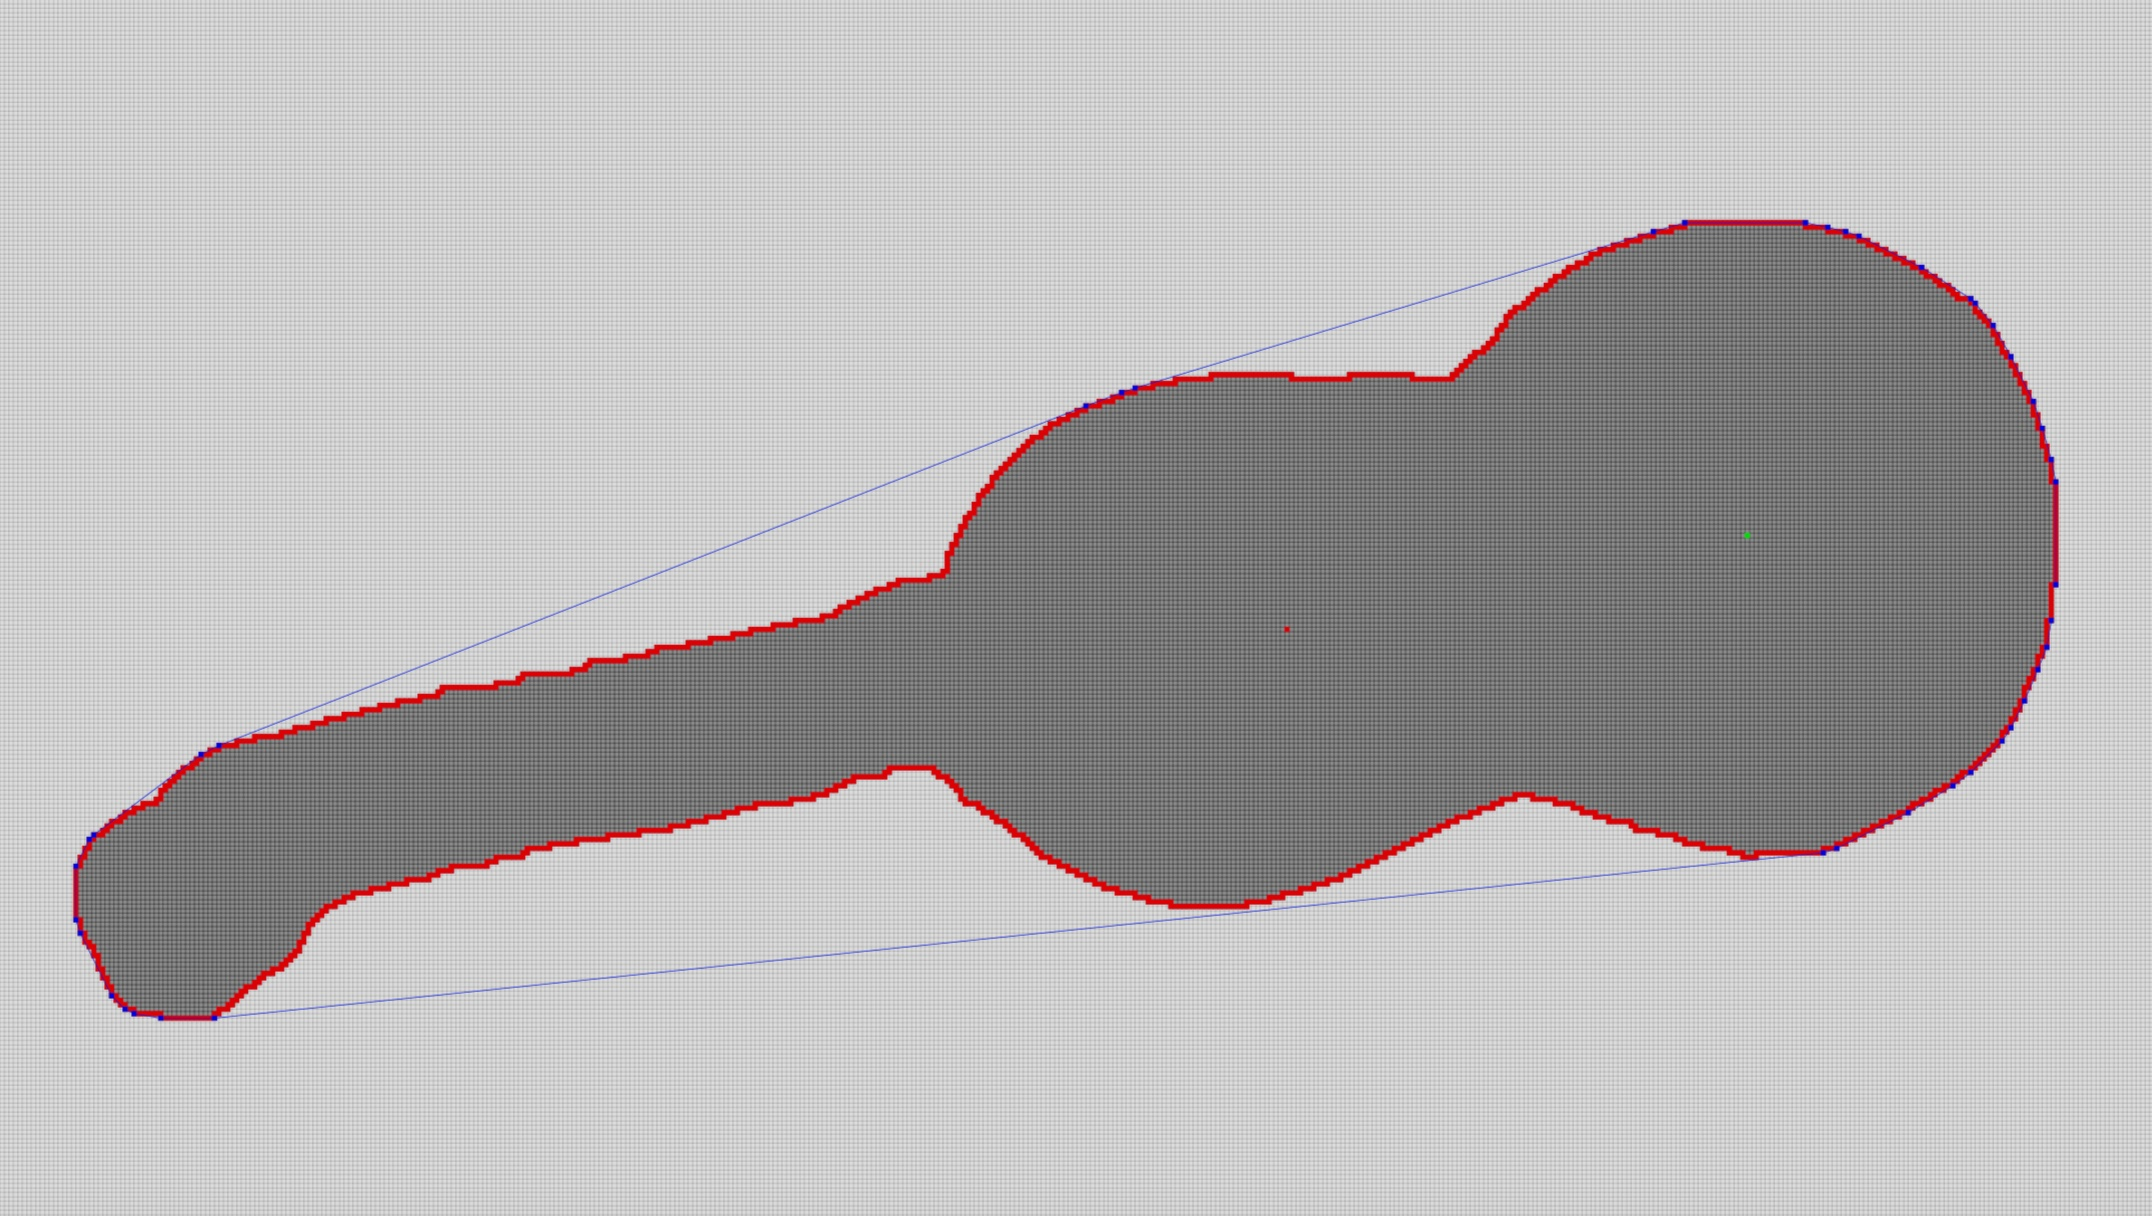
\includegraphics[scale=0.1]{guitar.pdf}
\section{PERIMETRE} Cet indicateur mesure la longueur du contour de l'image. Il est destiné à différencier les formes très courbés (tel lizzard) de celle qui se rapproche plus d'un disque (tel apple). Il est calculé en extrayant le contour de la forme avec la fonction $contour$ inplémentée dans le fichier $utils.cpp$. Le contour obtenu correspond a une topologie 4.
\subsection{Resistance au bruit}
Le contour est par nature assez sensible au bruit. 
En effet, le bruit se situant majoritairement au bord, c'est le contour qui est le premier modifié.
POur limiter ce problème, on ne garde que la plus grande composante connexe en topologie 4. Ainsi, même


L'orentation de notre figure n'a que très peu d'impact sur notre contour. 
Lorque la taille de l'image est assez grande, tourner l'image conserve la taille du contour même si à certain endroit particuliers,

\section{DISQUECIRCONS} : A Partir de la position du barycentre et de la distance du point le plus éloigné de celui-ci, calculé par les fonctions \textbf{barycentre} et \textbf{distFarthestPoint} dans \textbf{utils.cpp}, on calcule le rapport entre la surface du disque circonscrit à la forme et la surface de de la forme.
\section{NBSEG} : Le nombre de segment qui délimitent l'enveloppe convexe de l'image. Les points qui relient ces segments sont calculé par l'algorithme de Graham inplémenté par la fonction \textbf{convexHull} dans \textbf{convexhull.cpp}. Pour la première étape de l'algorithme où sont triés les points selon un ordre lié à un point \textbf{p0}, le tri n'a d'abord pas fonctionné car des points étaient alignés avec \textbf{p0}, mais ce problème a été corrigé en prenant en compte la distance avec celui-ci.
% todo : verifier algo
\section{MAXSEG} : Cet indicateur mesure la taille du plus grand segment délimitant l'enveloppe convexe.


\end{document}

